\documentclass{article}
\usepackage{tikz}
\usepackage{float}
\usepackage{enumerate}
\usepackage{amsmath}
\usepackage{amsthm}
\usepackage{bm}
\usepackage{indentfirst}
\usepackage{siunitx}
\usepackage[utf8]{inputenc}
\usepackage{graphicx}
\graphicspath{ {Images/} }
\usepackage{float}
\usepackage{mhchem}
\usepackage{chemfig}
\allowdisplaybreaks

\title{6.041 Problem Set 5}
\author{Robert Durfee - R02}
\date{October 10, 2018}

\begin{document}

\maketitle

\section*{Problem 1}

\textit{For each one of the following figures, identify if it corresponds to
a valid CDF. The value of the CDF at points of discontinuity is indicated
with a small solid circle.}

\subsection*{Part A}

\begin{center}
    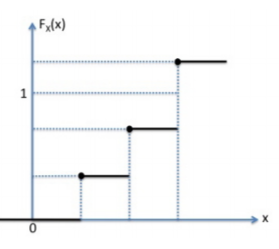
\includegraphics[scale=1]{Images/P1A.PNG}
\end{center}

This figure cannot correspond to a legitimate CDF as its maximum value is
greater than 1.

\subsection*{Part B}

\begin{center}
    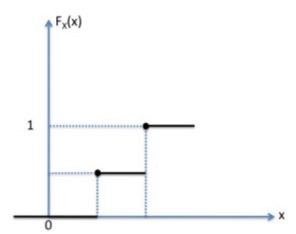
\includegraphics[scale=1]{Images/P1B.PNG}
\end{center}

This is a valid CDF.

\subsection*{Part C}

\begin{center}
    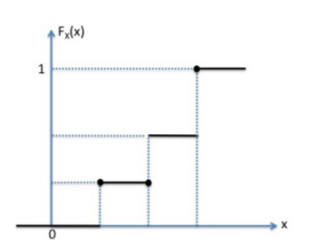
\includegraphics[scale=1]{Images/P1C.PNG}
\end{center}

This is not be a valid CDF because of the value of the second discontinuity.

\subsection*{Part D}

\begin{center}
    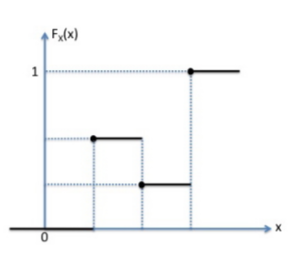
\includegraphics[scale=1]{Images/P1D.PNG}
\end{center}

This cannot be a valid CDF because it isn't monotonically increasing.

\section*{Problem 2}

\textit{Random variables $ X $ and $ Y $ are distributed according to the
joint PDF}
$$ f_{X,Y}(x, y) = \begin{cases}
    ax & \mathrm{if} \, 1 \leq x \leq 2 \, \mathrm{and} \, 0 \leq y \leq x \\
    0 & \mathrm{otherwise}
\end{cases} $$

\subsection*{Part A}

\textit{Find the constant $ a $.}

\subsection*{Part B}

\textit{Determine the marginal PDF $ f_Y(y) $.}

\section*{Problem 3}

\textit{Paul is vacationing in Monte Carlo. On any given night, he takes X
dollars to the casino and returns with Y dollars. The random variable X has
the PDF shown in the figure. Conditional on X = x, the continuous random
variable Y is uniformly distributed between zero and 2x.}

\begin{center}
    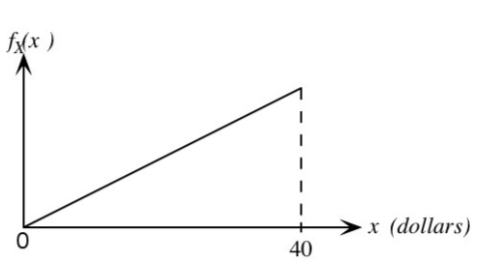
\includegraphics[scale=1]{Images/P3.PNG}
\end{center}

\subsection*{Part A}

\textit{Determine the joing PDF $ f_{X,Y}(x, y) $.}

\subsection*{Part B}

\textit{On any particular night, Paul makes a profit of $ Z = Y - X $ dollars.
Find the probability that Paul makes a positive profit (i.e., $ P(Z > 0)$). }

\subsection*{Part C}

\textit{Find the PDF of Z. Express your answers in terms of z.}

\subsection*{Part D}

\textit{Calculate the expected value of Z.}

\section*{Problem 4}

\textit{The figure below describes the joint PDF of random variables X and Y
. These random variables take values in $[0, 2]$ and $[0, 1]$, respectively.
At $x = 1$, the value of the joint PDF is $1/2$}

\begin{center}
    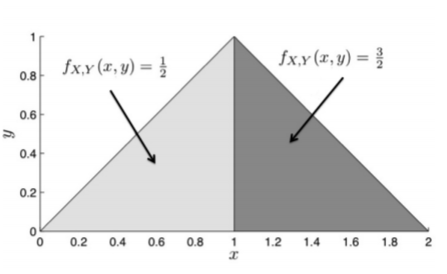
\includegraphics[scale=1]{Images/P4.PNG}
\end{center}

\subsection*{Part A}

\textit{Are X and Y independent?}

\subsection*{Part B}

\textit{Find $ f_X(x) $. Express your answers in terms of x.}

\subsection*{Part C}

\textit{Find $ f_{Y|X}(y \mid 0.5) $.}

\subsection*{Part D}

\textit{Find $ f_{X|Y}(x \mid 0.5) $.}

\subsection*{Part E}

\textit{Let $ R = XY $ and let $A$ be the event $ \{ X < 0.5 \} $. Evaluate $
E[R \mid A] $.}

\section*{Problem 5}

\subsection*{Part A}

\textit{Let X be a random variable that takes values between 0 and c, for
some $ c > 0 $, so that $P(0 \leq X \leq c) = 1$. Prove that $\mathrm{var}(X)
\leq c^2/4$.}

\subsection*{Part B}

\textit{Let X be a non-negative continuous random variable. Using the
definition $E[X] = \int_0^{\infty} x f_X(x) dx $, show that $ E[X] =
\int_0^{\infty} P(X > t) dt $.}

\end{document}